\section{Validierung}
In den folgenden Kapiteln werden die Validierungen der Spannungsmessung und die Konzepte für die Datenübertragung via Powerline, Fehlererkennung eines Moduls und der Kollisionserkennung erklärt.
\subsection{Datenübertragung auf Sensorprint}
Die Übertragung der Daten vom Analog-Digital-Converter zum Mikrocontroller wird anhand des SPI Übertragungsprotokolls gewährleistet. In Abbildung \ref{SPI_MISO} und \ref{SPI_MOSI} sind die übertragenen Werte erkennbar. 
\begin{figure}[htb]
\centering
\includegraphics[width=0.5\textwidth]{sections/data/singalbilder1.jpg}
\caption{MOSI: Mikrocontroller out ADC in}
\label{SPI_MOSI}
\end{figure}

\begin{figure}[htb]
\centering
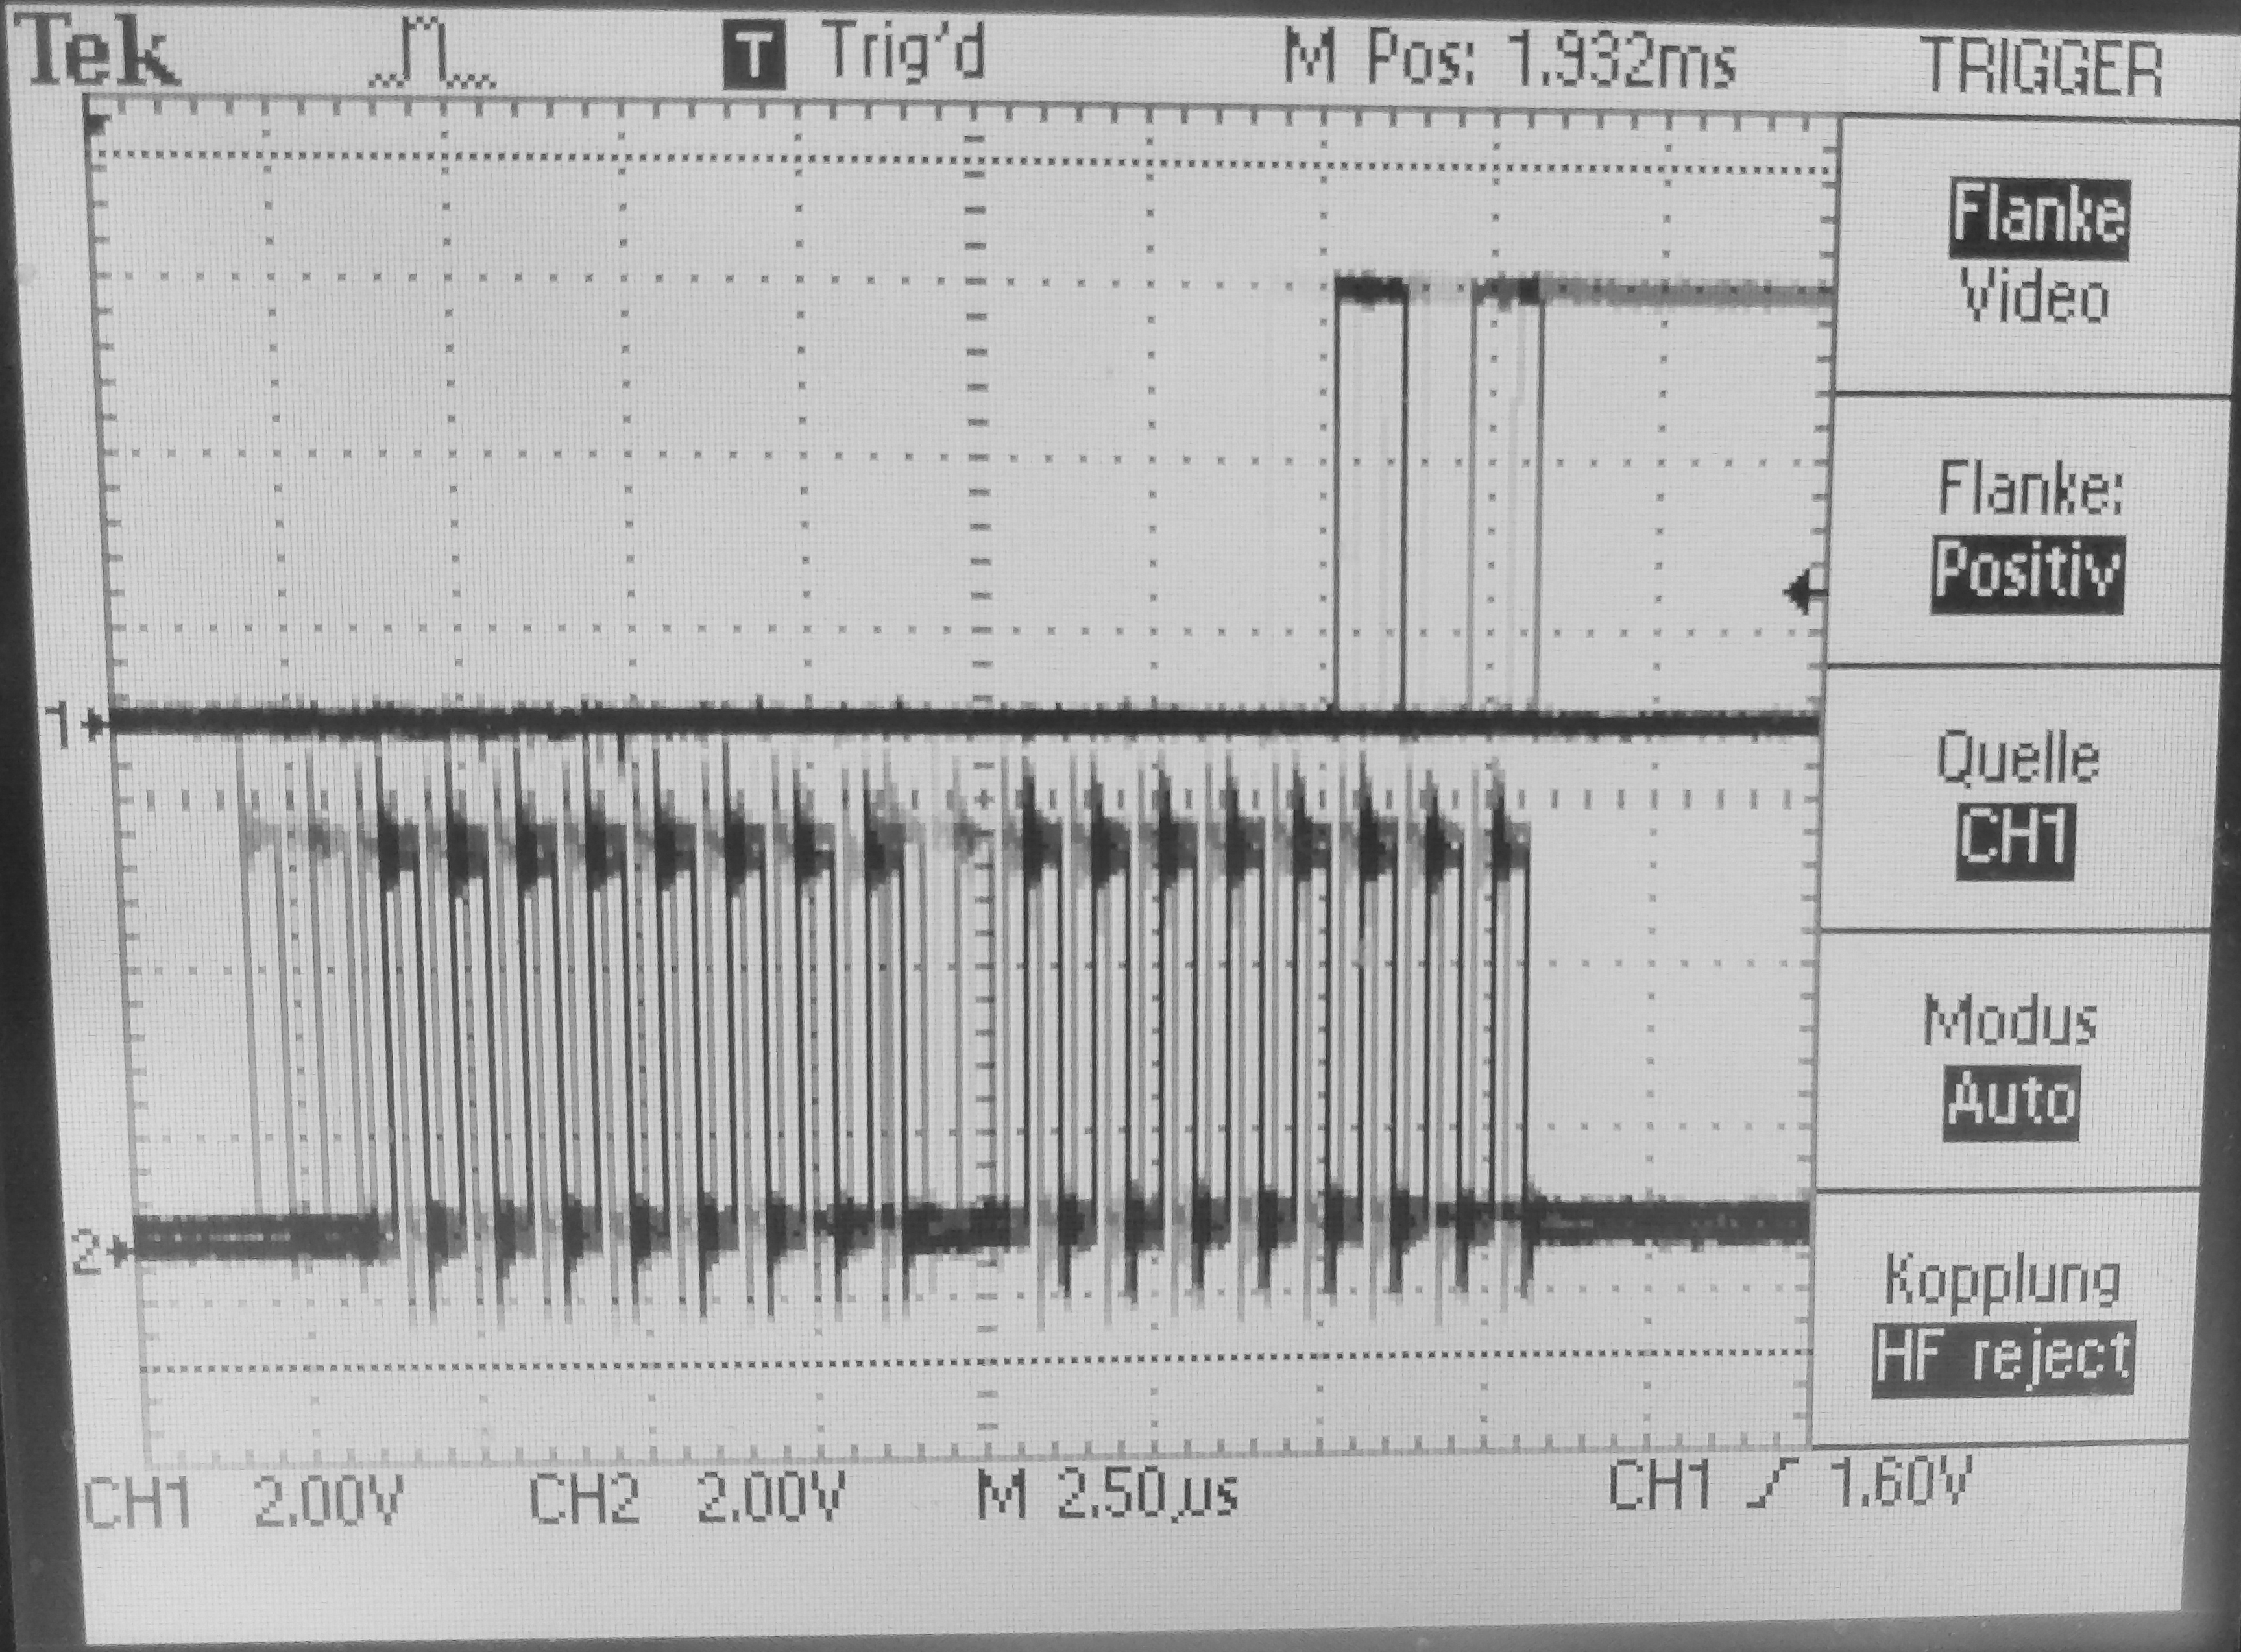
\includegraphics[width=0.5\textwidth]{sections/data/singalbilder3.jpg}
\caption{MISO: Rückgabewert von ADC}
\label{SPI_MISO}
\end{figure}

Wie in den vorhergehenden Abbildungen ersichtlich, funktioniert die Kommunikation zwischen ADC und Mikrocontroller, denn der ADC gibt ein Bitmuster zurück, welches mit der in Abschnitt \ref{Spannungsmessung} beschriebenen Software verwendet werden kann. \\
\newpage
Die Kommunikation zwischen Mikrocontroller und Tranceiver funktioniert via UART. Die folgenden Abbildungen \ref{Trans_Ein} und \ref{Trans_Aus} die Übertragung.
\begin{figure}[htb]
\centering
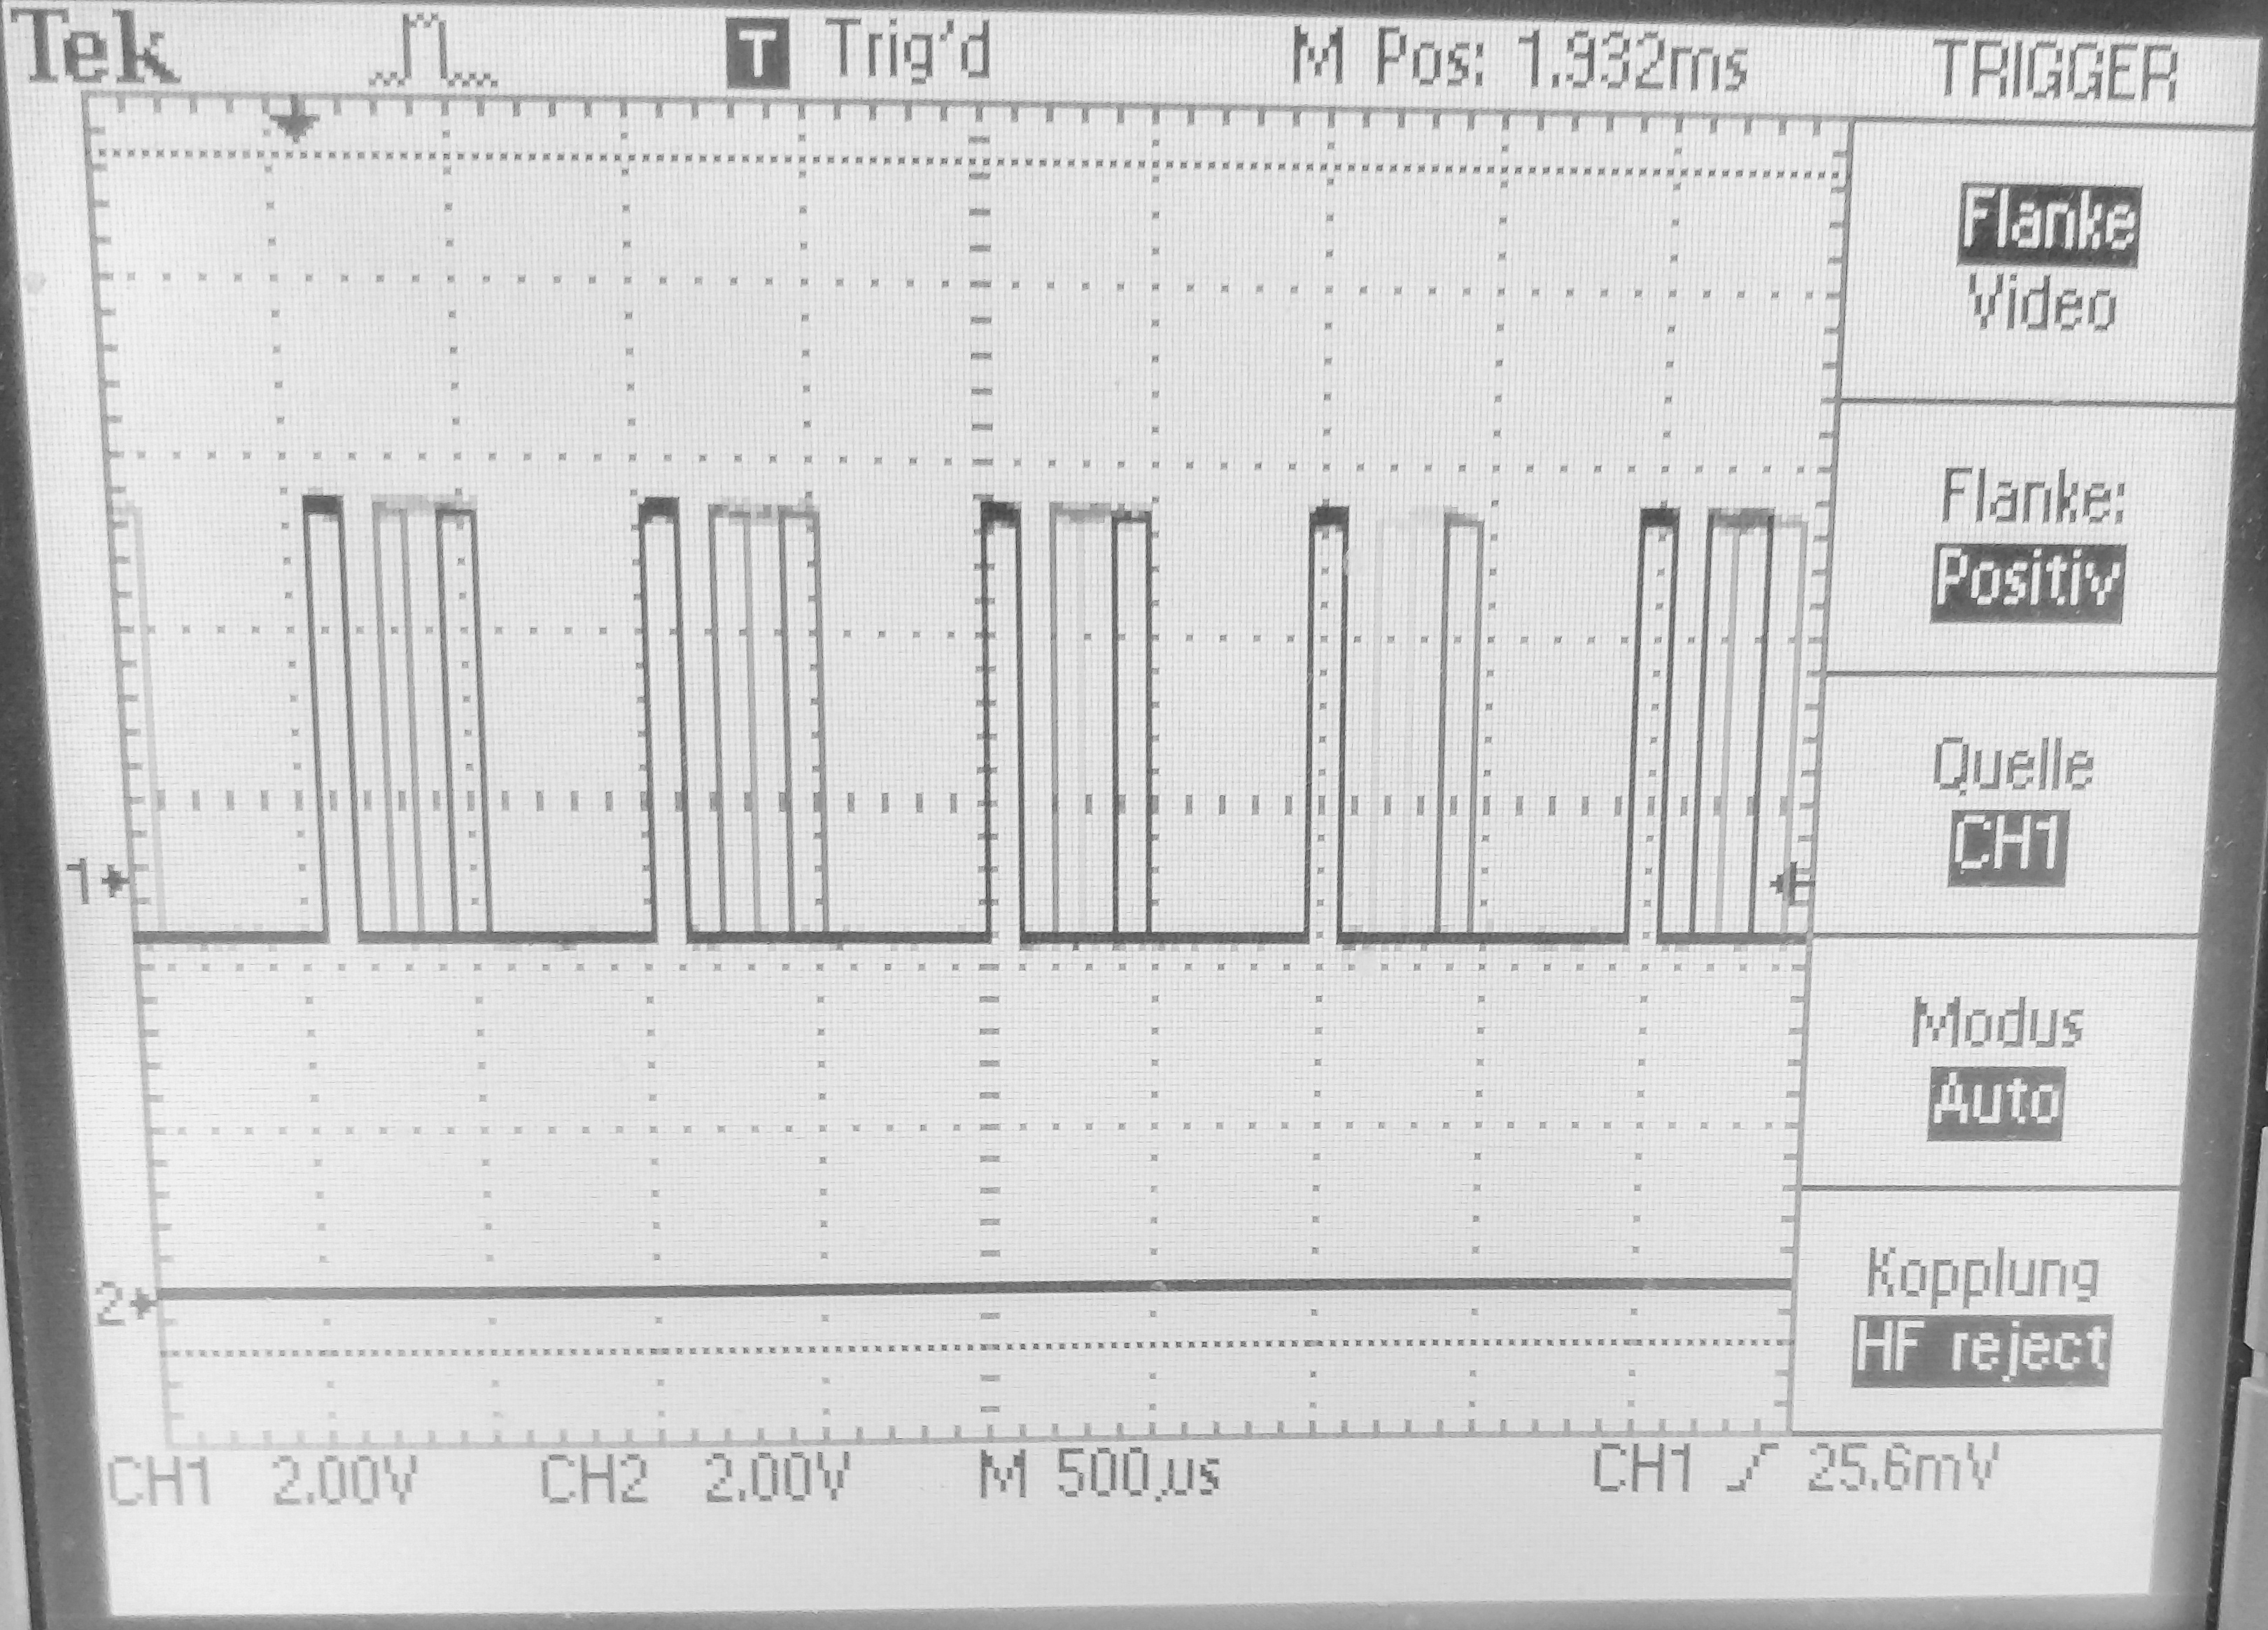
\includegraphics[width=0.5\textwidth]{sections/data/singalbilder8.jpg}
\caption{Tranceiver Eingang}
\label{Trans_Ein}
\end{figure}

\begin{figure}[htb]
\centering
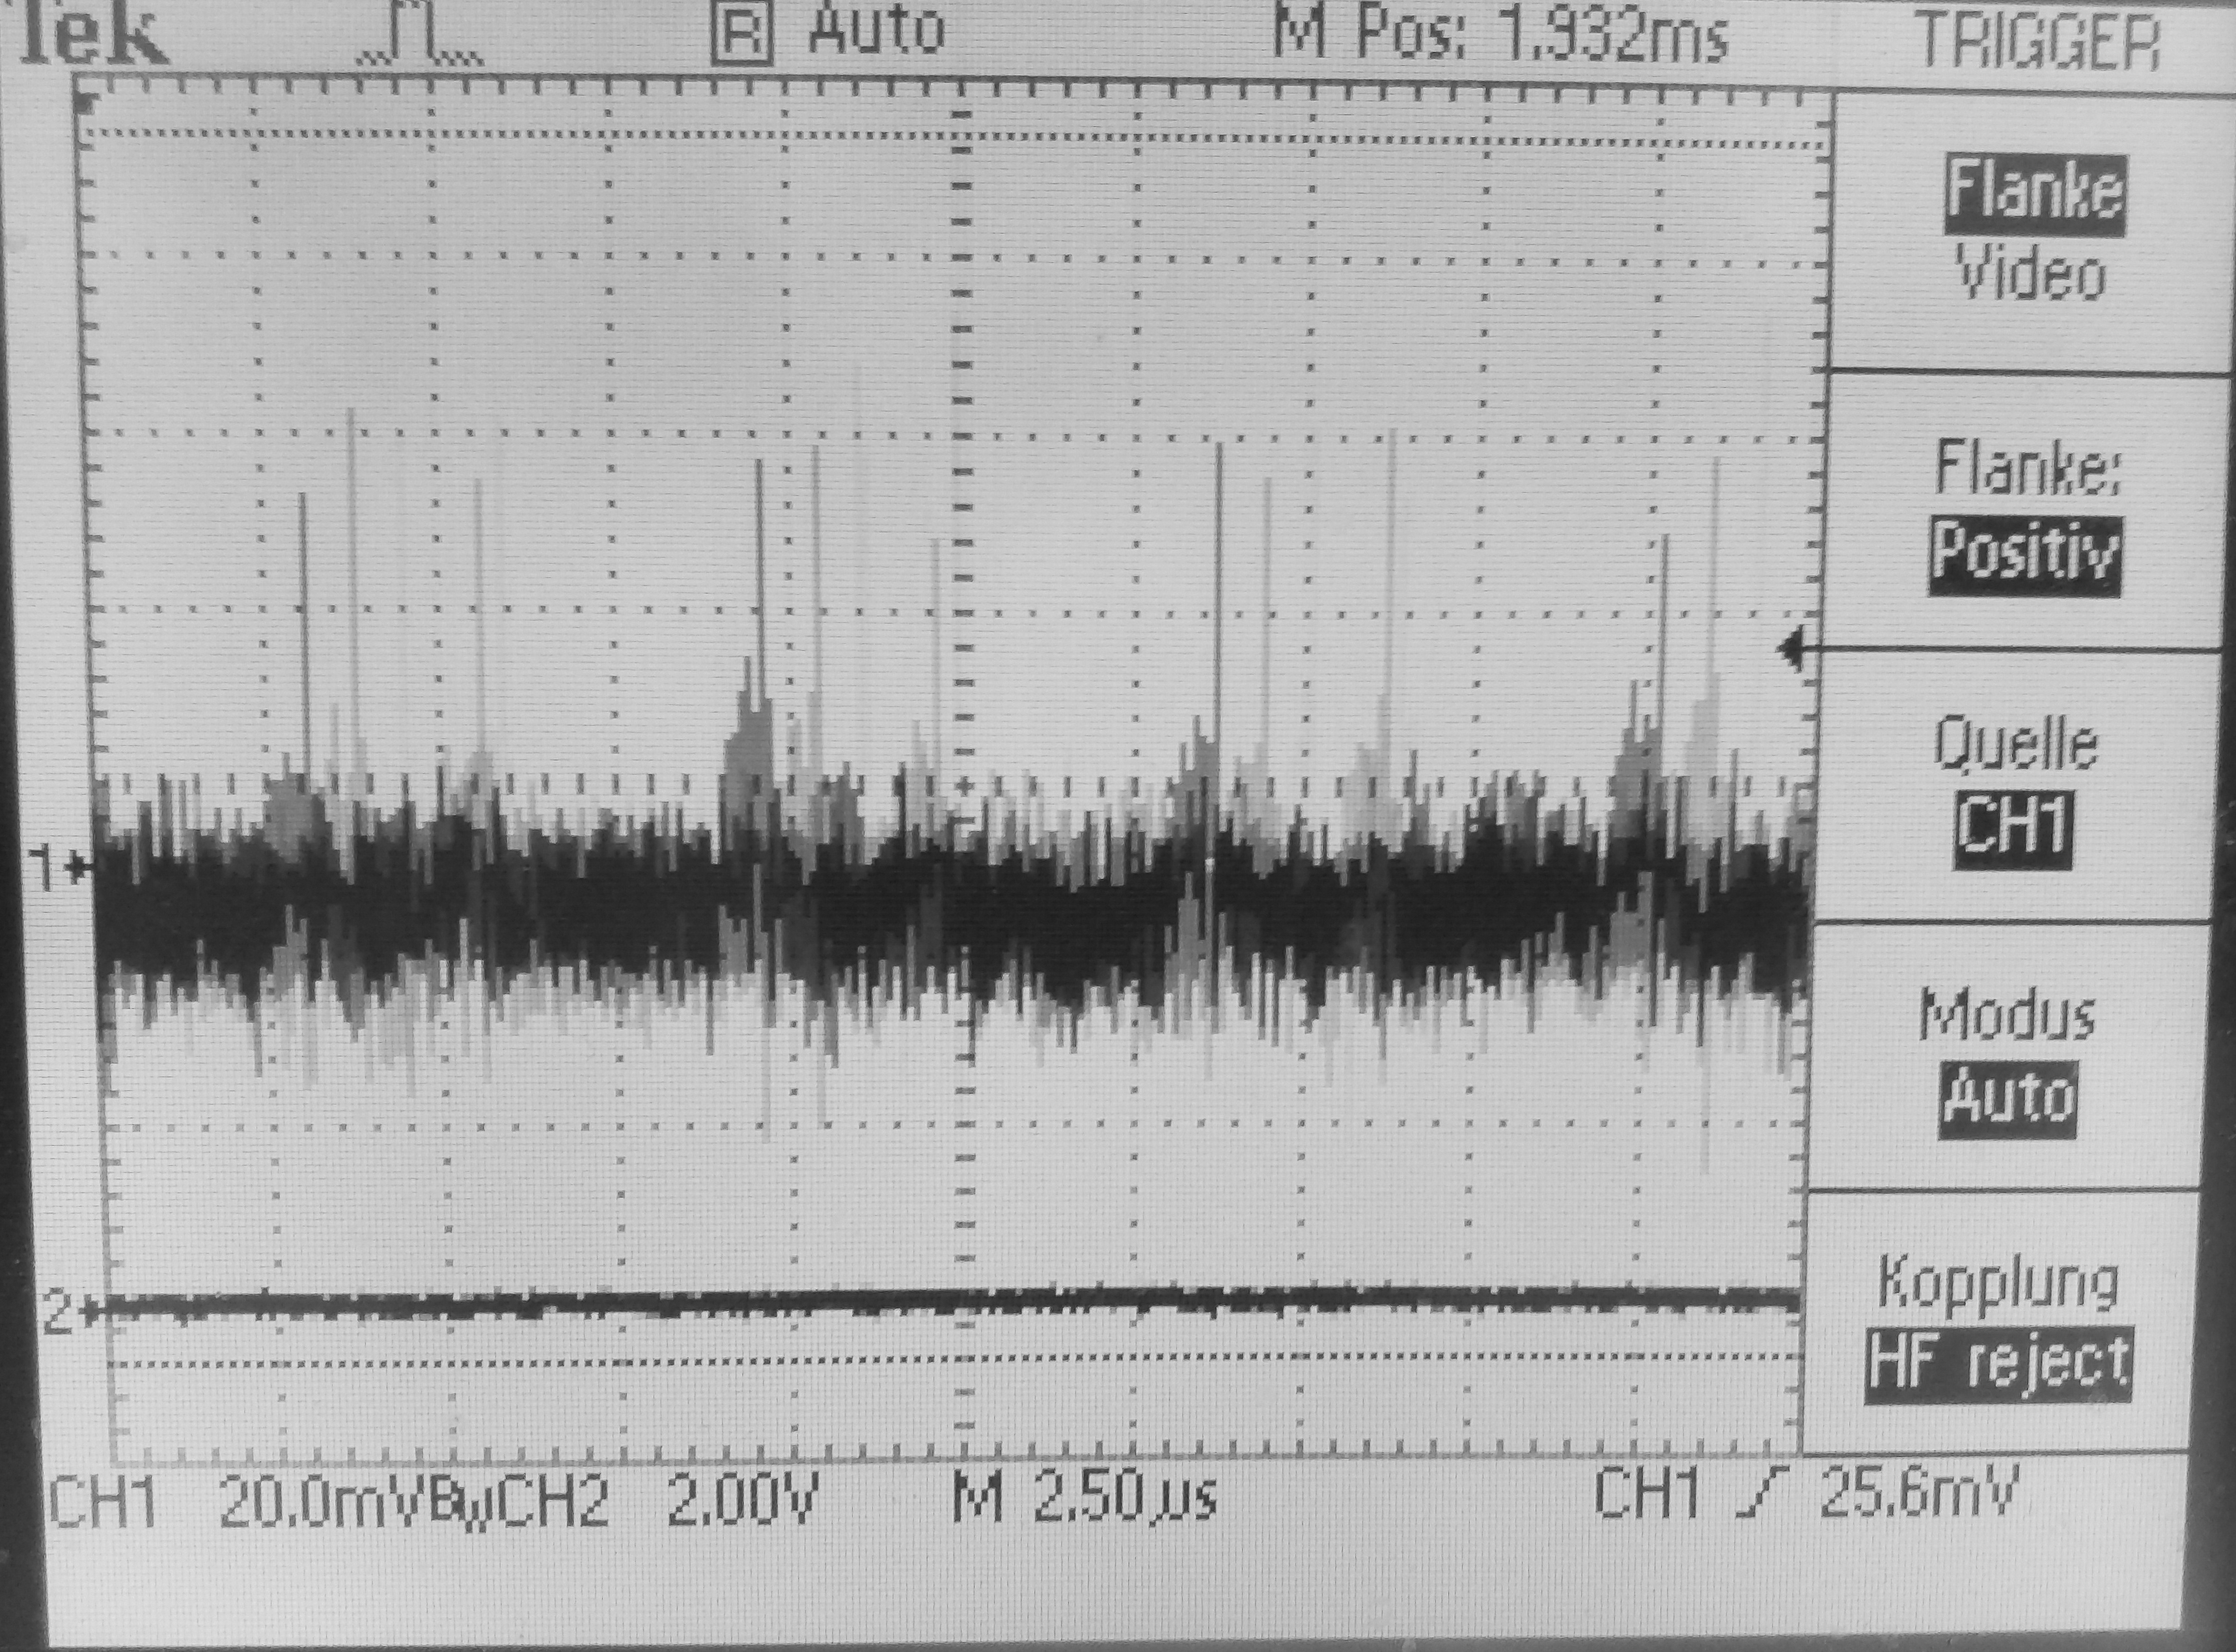
\includegraphics[width=0.5\textwidth]{sections/data/singalbilder4.jpg}
\caption{Tranceiver Ausgang}
\label{Trans_Aus}
\end{figure}


\subsection{Spannungsmessung}
Als Indiz für eine defekte oder verdunkelte Solarzelle wird die Zellenspannung gemessen, daher ist bei dieser die Messgenauigkeit sehr wichtig und wurde vom Auftraggeber auf $\pm$0.1V festgelegt. Um dies zu überprüfen, wird die angelegte Spannung mit einem weiteren Messgerät aufgezeichnet und mit dem ermittelten Wert verglichen. \\
Die Spannungsmessung soll softwaremässig, wie in Abschnitt \ref{Spannungsmessung} beschrieben, gelöst werden. Die Genauigkeit soll mit einem Spannungsgenerator als Quelle überprüft werden. 
\subsection{Datenübertragung via Powerline}
Das Ziel dieser Messung ist es, eine vorher definierte Anzahl Bits via Powerline zu übertragen. Dafür werden an einem spannungsführenden Kabel zwei Ferritkerne, mit verschiedenen Abständen dazwischen, angebracht und über eine Spule mit dem jeweiligen Transceiver verbunden. Das vom ersten Transceiver gesendete Bitmuster sollte beim zweiten Transceiver empfangen werden und das selbe Bitmuster wird wieder ausgeben.
Die Abstände werden wie folgt verändert und das Empfangen von Bitmuster überprüft:
\begin{enumerate}
\item[•]1 m
\item[•]10 m
\item[•]25 m
\item[•]50 m
\item[•]100 m
\end{enumerate}
Dieses Testkonzept gewährleistet eine ganzheitliche Überprüfung des Empfanges, sowohl bei kleinen als grossen Solaranlagen.
\subsection{Fehlererkennung eines Moduls}
Damit eine einfache Lokalisierung des defekten Moduls sichergestellt ist, hat jeder Sensorprint eine eigene Erkennungsnummer. Um sicher zu stellen, dass diese Erkennungsnummer korrekt übertragen und verarbeitet wird, ist ein einfaches Testkonzept vorgesehen. Das Sensorboard wird auf eine gewisse Erkennungsnummer eingestellt und der Meldeprint kalibriert. Anschliessend wird die Nummer geändert was zur Folge hat, dass der Meldeprint einen Fehler ausgibt und diesen auf dem LCD-Display mit der dazugehörigen Erkennungsnummer anzeigt. Im folgendem Kapitel sind die Ergebnisse dieses Tests aufgeführt.
\subsection{Kollisionserkennung}
Alle Mikrocontroller senden ihre Daten in einem vorher festgelegten Zeitintervall, dadurch kommt es zu Kollisionen. Um sicherzustellen, dass der Meldeprint nur mit korrekt übertragenen Messwerten rechnet, werden zusätzliche Informationen gesendet. Überprüft wird diese CRC genannte Methode indem die Übertragung vorzeitig unterbrochen wird. Der Mikrocontroller sollte damit in der Lage sein, das fehlerhafte Packet zu erkennen und dieses zu ignorieren. Die Resultate dieser Messung sind in diesem Kapitel aufgeführt.